\chapter{Implementación del software\label{sec:Implementacion_soft}}

Una vez finalizado el soporte físico del sistema, será necesario implementar a nivel de software todas las funciones deseadas.

El sistema está compuesto por tres microcontroladores, cada uno de ellos con sus propias características y métodos de programación. Debido a esto, a lo largo de este capítulo se explicará con detenimiento el software utilizado individualmente para ellos así como los distintos entornos de desarrollo (\acrshort{IDE}) necesarios.

Los distintos elementos se presentarán siguiendo el mismo orden que la información que se desea adquirir. Este es:
ADS $\Rightarrow$ Microcontrolador $\Rightarrow$ Interfaz inalámbrica $\Rightarrow$ PC.

\section{Microcontrolador STM32F4\label{sec:Software_micro}}

Debido a la complejidad de los microcontroladores de la familia STM32, los desarrolladores han dedicado su tiempo y esfuerzo en crear herramientas que faciliten su programación. Estas herramientas llamadas \acrshort{IDE} contienen una recopilación de funciones, utilidades y ejemplos que simplifican sensiblemente el proceso de diseño e implementación del software que ejecutará el microcontrolador.

Es tan grande la comunidad de desarrolladores que hay detrás del STM que numerosas empresas han visto como una oportunidad de negocio la creación de un \acrshort{IDE} propietario.

\clearpage

\begin{figure} [h]
    \centering
    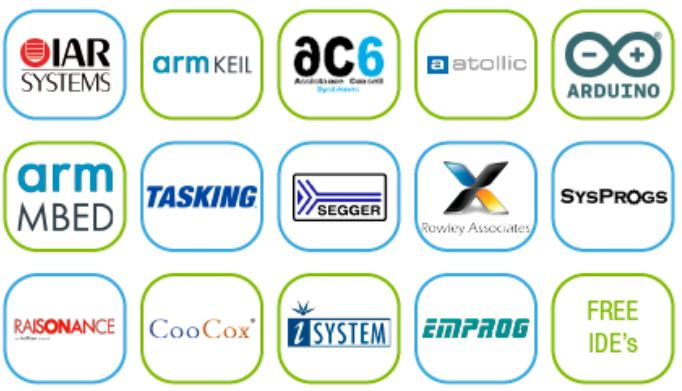
\includegraphics[width=13cm]{STM32_IDEs}
    \caption{IDEs alternativos disponibles \cite{STM32_IDEs}}
    \label{fig:STM32_IDEs}
\end{figure}

La figura \ref{fig:STM32_IDEs} muestra algunos entornos de desarrollo recomendados por el fabricante en su propia página web. Como se puede apreciar, en la imagen se hace distinción entre las opciones comerciales (azul) y las gratuitas (verde).

Uno de los objetivos de este proyecto era utilizar Software Libre en la medida de lo posible. Por ese motivo se probaron algunas de las alternativas presentes en la imagen anterior dando preferencia a aquellas basadas en Oracle como ``System Workbench for STM32'' (AC6). A continuación se presentan algunas de las utilizadas al comienzo del proyecto junto con sus características y el motivo de su descarte:
\begin{itemize}
   \item \textbf{CooCox}\\
   Presenta muchos ejemplos prácticos pero su interfaz es muy lenta. Necesita demasiado tiempo para iniciar.
   \item \textbf{Arduino}\\
   Fase muy temprana de desarrollo.
   \item \textbf{System Workbench for STM32}
   \\Buena comunidad pero incompatible con las herramientas de STM.
\end{itemize}

\begin{figure} [h]
    \centering
    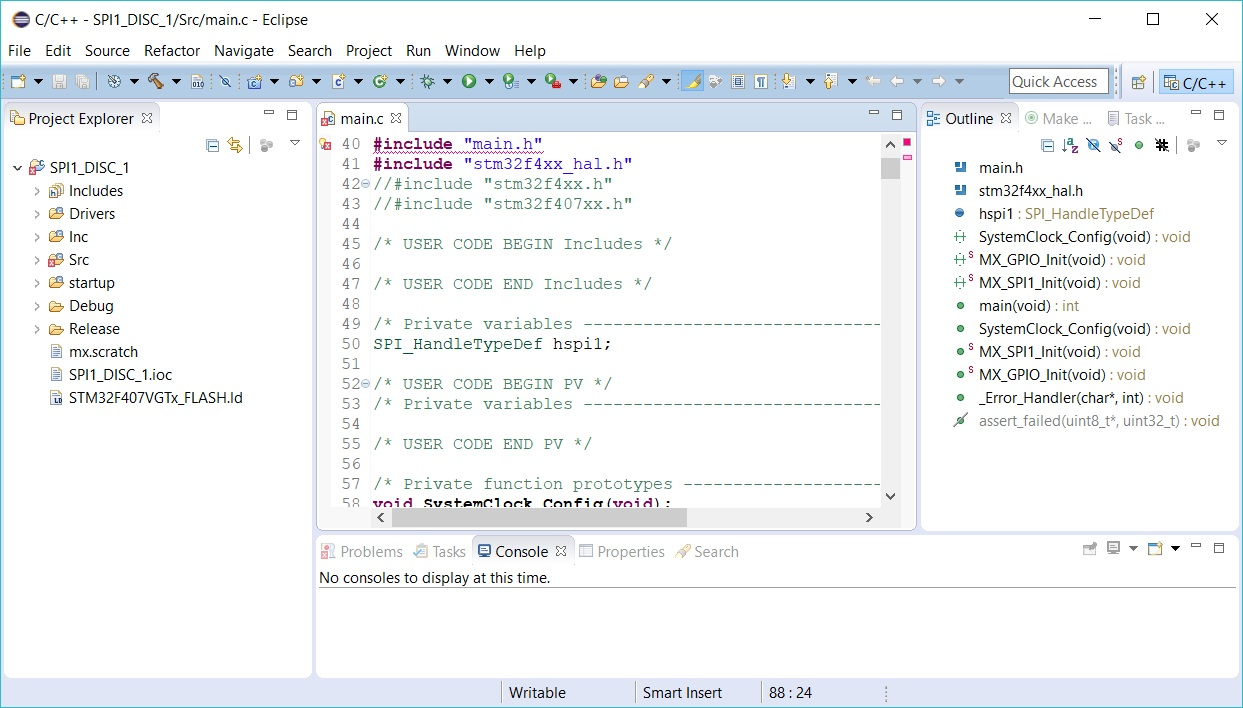
\includegraphics[width=12cm]{Alternative_IDE}
    \caption{Ejemplo de IDE alternativo}
    \label{fig:Alternative_IDE}
\end{figure}

Finalmente se optó por armKeil, pues tiene una gran cantidad de ejemplos y librerías descargables desde la propia interfaz, contiene un gran número de funciones adicionales y la compatibilidad con las herramientas de STM es muy buena. Aunque en la figura \ref{fig:STM32_IDEs} aparece entre las alternativas gratuitas se debe destacar que cuenta con dos versiones, una gratuita que permite realizar proyectos básicos y otra comercial destinada a aplicaciones de mayor envergadura. La limitación de la versión gratuita consiste en forzar un tamaño máximo de programa de 32KB. Si el código a compilar supera dicha longitud directamente no compilará.

\subsection{Configuración inicial\label{sec:Configuracion_micro}}

Aunque Keil permite comenzar un proyecto utilizando como base algunos de los ejemplos que contiene, la configuración de las características del microcontrolador (reloj, interfaces, etc.) puede resultar una tarea muy compleja y tediosa, incluso para aquellos desarrolladores más experimentados. Con el objetivo de facilitar esta tarea, el fabricante ha creado un software con interfaz amigable que permite configurar de forma gráfica el procesador llamado STM32CubeMX que hace uso de un conjunto de elementos y \textit{drivers} llamado \acrshort{HAL} que se explicará con más detalle al comienzo del apartado \ref{sec:Software_micro_HAL}.

\begin{figure} [h]
    \centering
    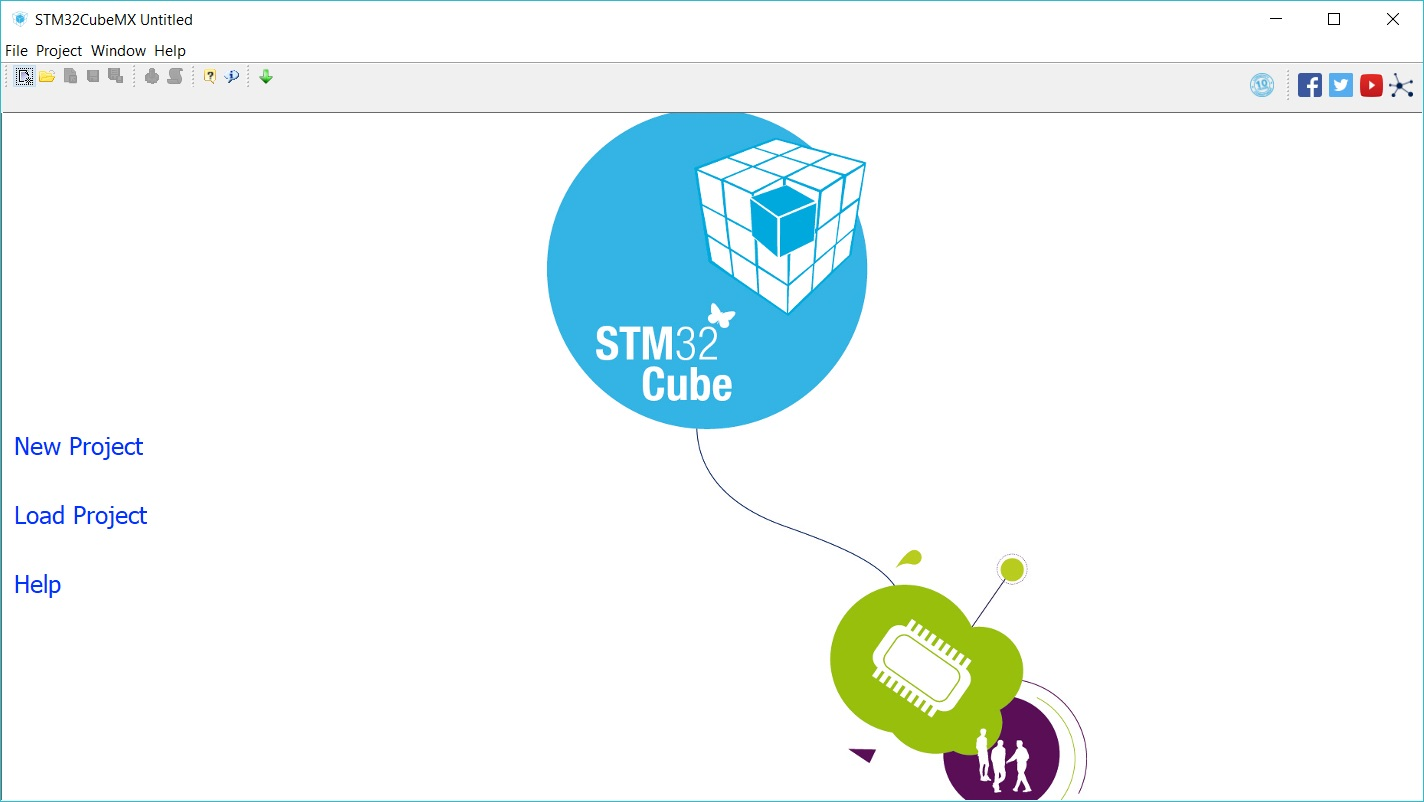
\includegraphics[width=11cm]{STM32CubeMX}
    \caption{Inicializador de proyectos STM32CubeMX}
    \label{fig:STM32CubeMX}
\end{figure}

La herramienta STM32CubeMX incluye una base de datos de todos los microcontroladores disponibles, permitiendo seleccionar el formato, encapsulado e incluso si se va a utilizar en su formato nucleo o en un kit de desarrollo. Incluye también documentación sobre cada microcontrolador y enlaces a distribuidores en caso de que el usuario final quiera comprarlo. 

\subsubsection{Asignación de funciones\label{sec:Configuracion_micro_asignacion}}

Tras seleccionar el microcontrolador, se presenta al usuario una zona de trabajo dividida en cuatro pestañas, cada una destinada a configurar un conjunto de características del microcontrolador: pines y sus funciones, reloj, interfaces de comunicación y consumo de energía.

\begin{figure} [h]
    \centering
    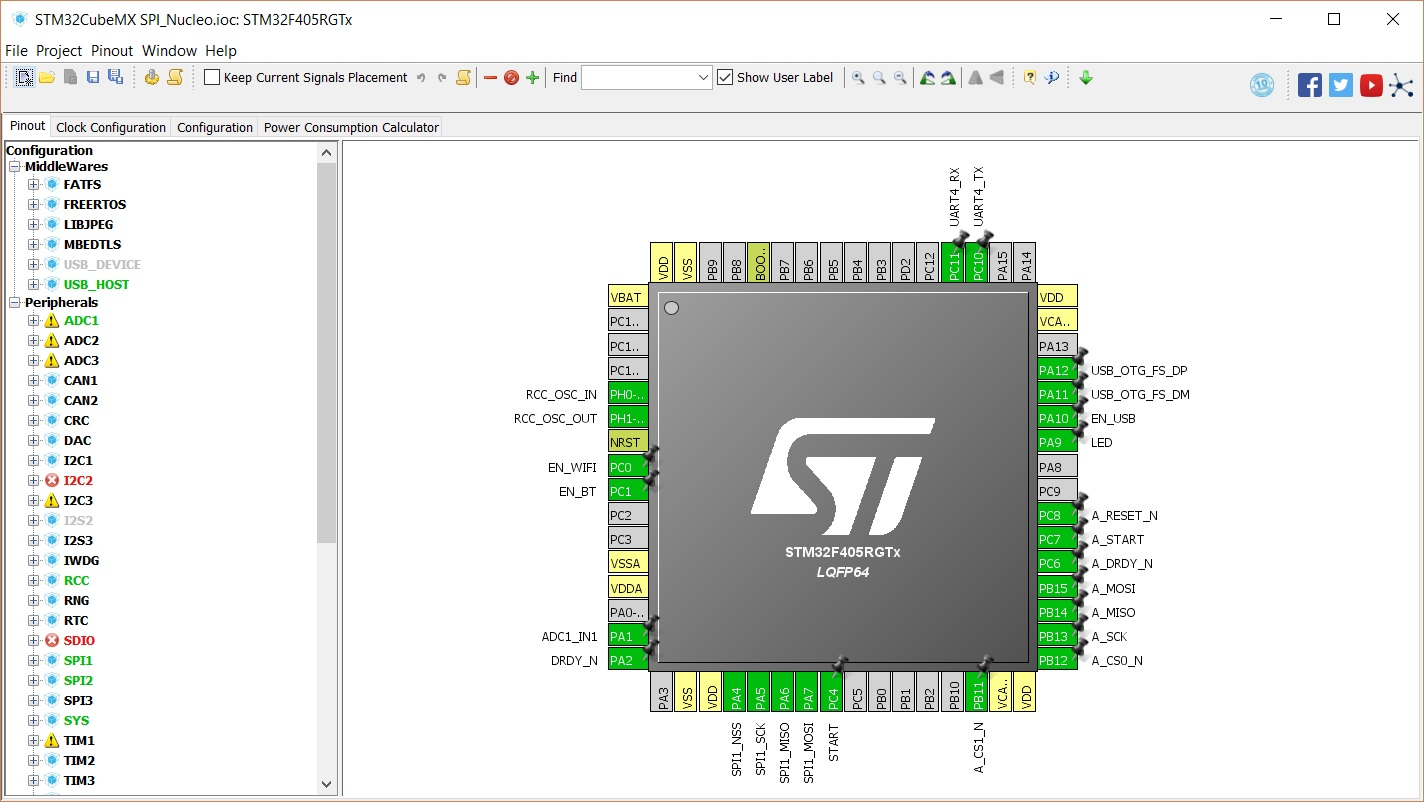
\includegraphics[width=15cm]{STM32CubeMX_pin}
    \caption{Espacio de trabajo del STM32CubeMX}
    \label{fig:STM32CubeMX_pin}
\end{figure}

La configuración de pines permite, no sólo ver de forma visual cada una de las funciones alternativas de cada pin, sino que además indica si alguna no está disponible y las alternativas si se da el caso.

En la figura \ref{fig:STM32CubeMX_pin} aparece la configuración utilizada en este proyecto. En la imagen se puede apreciar que todas las interfaces necesarias para llevar a cabo este proyecto ya han sido asociadas a su pin correspondiente y aún quedan libres casi la mitad de los pines. Esto es un indicador de la versatilidad de este dispositivo.

\subsubsection{Configuración de los relojes\label{sec:Configuracion_micro_reloj}}

Este apartado es el más importante, pues un reloj mal configurado puede provocar errores en la comunicación, una mala gestión del tiempo e incluso que el propio microcontrolador no arranque.

La interfaz desarrollada por STM muestra de forma visual todos los relojes que intervienen en el dispositivo así como las relaciones que hay entre ellos. De esta forma basta con seguir las líneas que conectan los distintos tipos de reloj para saber las dependencias que existen y los resultados que obtendrán en función de los valores escogidos.
\\En caso de que alguna configuración sea incorrecta la propia herramienta está preparada para ofrecer una solución que se acerque lo máximo posible a los resultados deseados.

\begin{figure} [h]
    \centering
    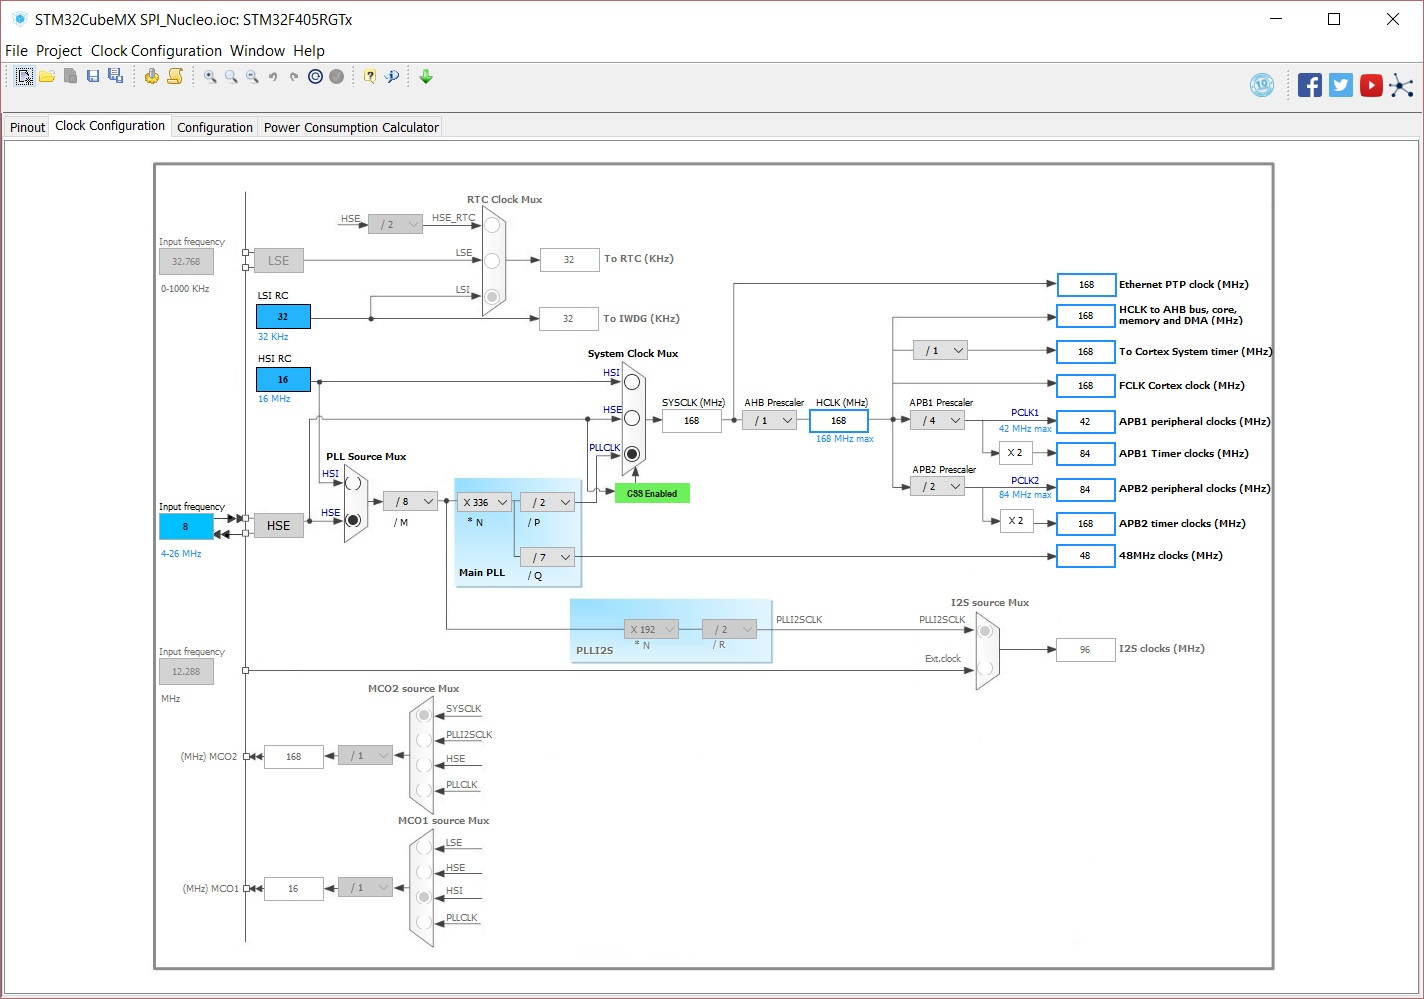
\includegraphics[width=15cm]{STM32CubeMX_clock}
    \caption{Configuración del reloj del microcontrolador}
    \label{fig:STM32CubeMX_clock}
\end{figure}

En la figura \ref{fig:STM32CubeMX_clock} representa la configuración aplicada al microcontrolador durante la realización de este proyecto. A la izquierda se muestran distintas fuentes disponibles mientras que a la derecha se ve la frecuencia final de reloj resultante en cada una de las partes del microcontrolador (periféricos, temporizadores, memoria, etc).

Como se puede ver, aprovecha ambos osciladores, el externo (\acrshort{HSE} = 8MHz) y el interno (\acrshort{LSI} = 16MHz) para, usando \acrshort{PLL}, generar un reloj de una frecuencia mucho más elevada (168 MHz). Dicha frecuencia es, según el fabricante, la máxima frecuencia alcanzable por el dispositivo.

La función \acrshort{CSS} garantiza que, en caso de fallo del reloj del microcontrolador, este generará una alerta y entrará en un modo seguro. Esta función es muy útil cuando se está trabajando con elementos en los que la seguridad de las personas depende directamente del correcto comportamiento microcontrolador.

\clearpage

\subsubsection{Configuración de los periféricos\label{sec:Configuracion_micro_com}}

La tercera pestaña permite configurar los periféricos, esto incluye interfaces de comunicación, puertos GPIO, USB, etc.

\begin{figure} [h]
    \centering
    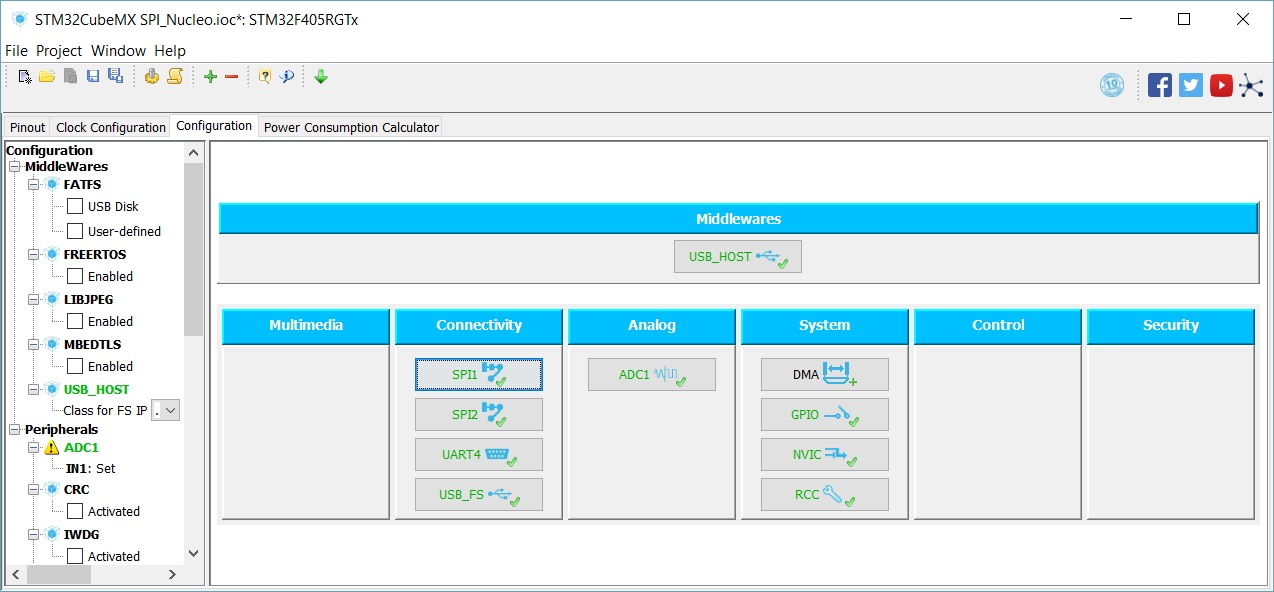
\includegraphics[width=15cm]{STM32CubeMX_conf}
    \caption{Configuración de las interfaces de comunicación}
    \label{fig:STM32CubeMX_conf}
\end{figure}

En función del estado del periférico, este aparecerá marcado con un \textit{tick} verde indicando que todo está correctamente configurado o una cruz roja avisando que alguna característica podría no estar disponible. Además será posible modificar la mayoría de las opciones relacionadas con ese periférico de forma intuitiva. 

\begin{figure} [h]
    \centering
    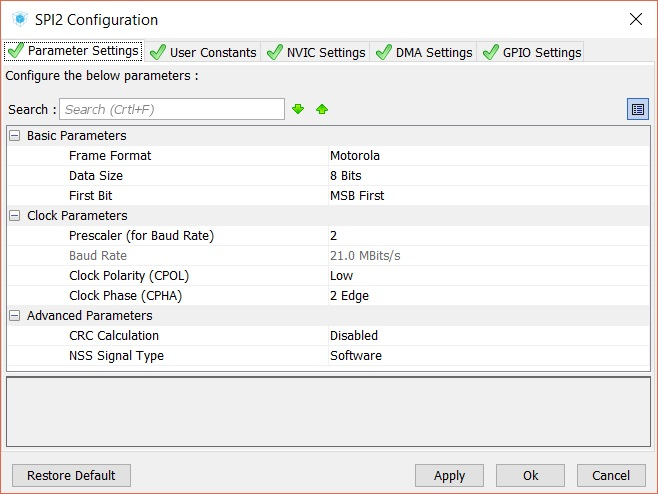
\includegraphics[width=10cm]{STM32CubeMX_conf_2}
    \caption{Detalle de la configuración de las interfaces de comunicación}
    \label{fig:STM32CubeMX_conf_2}
\end{figure}

En la figura \ref{fig:STM32CubeMX_conf_2} se muestran las opciones seleccionadas para el SPI que se comunicará con el los ADS. Se puede cambiar la velocidad, el modo de transmisión e incluso si la gestión del pin ``\textit{Chip-Select}'' se realizará de forma automática o manual.

\subsubsection{Calculo de consumo\label{sec:Configuracion_micro_consumo}}

La última pestaña, ``\textit{Power Consuption Calculator}'', contiene numerosas opciones para el análisis del consumo del microcontrolador. En esta se puede estimar la duración de la batería en función de parámetros como el modo funcionamiento, el tipo de fuente de alimentación e incluso la temperatura.

\begin{figure} [h]
    \centering
    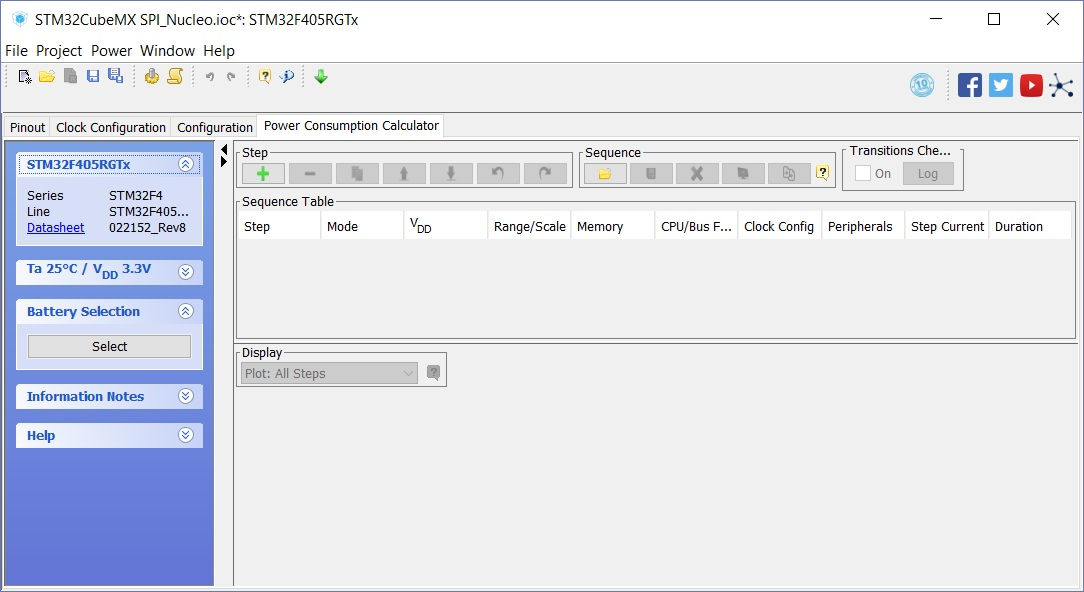
\includegraphics[width=15cm]{STM32CubeMX_otro}
    \caption{Calculadora del consumo del microcontrolador}
    \label{fig:STM32CubeMX_otro}
\end{figure}

\subsubsection{Generar código\label{sec:Configuracion_micro_generador}}

Finalmente es el momento de seleccionar el IDE para el cual el STM32CubeMX debe generar la base de código sobre la que se construirá el proyecto.

Esta herramienta es capaz de crear un código base para casi cualquier \acrshort{IDE} pero tras un par de usos queda claro que, de entre todos los disponibles, es armKeil con el que la integración da mejores resultados. La herramienta crea el código base con la configuración seleccionada desde la interfaz y lo integra dentro de un proyecto ya configurado y listo para trabajar.

Es importante destacar que la utilización de STM32CubeMX no sólo está pensada para facilitar el comienzo del diseño proporcionando una base sobre la que trabajar, también permite una mayor portabilidad del código ya que, si se siguen las reglas de programación sugeridas por la aplicación, esta permite realizar cambios de la configuración de los pines, los periféricos e incluso de familia de microcontrolador, todo ello sin necesidad de reestructurar el código.

\clearpage

El código que se ejecuta en el STM está dividido en dos fases. La primera, denominada comúnmente \textit{setup}, sólo se ejecuta la primera vez que se enciende el microcontrolador.
En esta se suelen declarar todas las variables globales, inicializar los periféricos y, en definitiva, preparar el microcontrolador para funcionar.

La segunda fase, denominada \textit{loop} es, como su nombre indica, un bucle infinito. En esta fase se ejecuta todo el código de forma cíclica. Normalmente en esta fase se incluye el funcionamiento normal del sistema, utilizando condicionales para forzar el comportamiento esperado.

Al generar el proyecto, el STM32CubeMX estructura el código tal como se muestra en el código \ref{algoritmo:Auto_gen}, dejando al usuario ciertas zonas libres para escribir en ellas y restringiendo la escritura en otras.

\begin{lstlisting}[label=algoritmo:Auto_gen,style = STM-code,frame=single,caption=Ejemplo de generación de código automáticamente]
  /* USER CODE BEGIN 1 */
	
  /* USER CODE END 1 */

  /* MCU Configuration----------------------------------------*/

  /* Reset of all peripherals, Initializes the Flash interface and the Systick. */
  HAL_Init();

  /* USER CODE BEGIN Init */

	
  /* USER CODE END Init */
\end{lstlisting}

Respetar dichas restricciones es opcional, pero en caso de no hacerlo no se podrá volver a cambiar la configuración original del micro mediante el STM32CubeMX, pues dicha herramienta las utiliza como referencia y no respetarlas puede ocasionar la pérdida del trabajo.

Por simplicidad, comodidad y compatibilidad, durante la realización de este trabajo se han respetado dichas restricciones construyendo todo el código en las zonas habilitadas para ello.

\clearpage

\subsection{Implementación del firmware \label{sec:Software_micro_HAL}}

A lo largo de las siguientes páginas se presentará una introducción a los elementos software utilizados, haciendo especial hincapié en aquel código cuya función es indispensable para cumplir con las especificaciones fijadas al comienzo del proyecto.

\subsubsection{HAL \label{sec:Software_micro_HAL}}

La programación de microcontroladores basados en Arduino y su \acrshort{IDE} resulta especialmente intuitiva ya que desde sus comienzos ese era uno de los objetivos: acercar el mundo analógico y digital a gente poco iniciada.

Los ARM de STM en cambio, están destinados a personas con cierta experiencia programando controladores. Permiten libertad total, proporcionando acceso a los registros sin restricciones y un control del hardware muy preciso. Si bien esta aproximación aumenta las posibilidades de la plataforma, también limita al número de personas que pueden ponerse a programar en ella así como la portabilidad de código.
\\Cuanto más cercano sea al hardware mayor exclusivo será y, por lo tanto, más cambios serán necesarios para portar dicho código a otra familia si en el futuro las especificaciones varían o se desean mejorar las características del sistema.

Con esta problemática en mente los desarrolladores de STM crearon un conjunto de herramientas y drivers que reciben el nombre de Hardware Abstraction Layer (\acrshort{HAL}).

\begin{figure} [h]
    \centering
    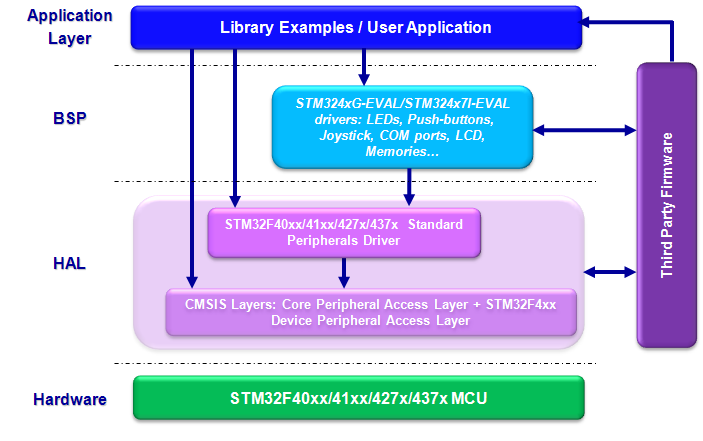
\includegraphics[width=13cm]{HAL-LL}
    \caption{Resumen del funcionamiento y características del HAL \cite{HAL-LL}}
    \label{fig:HAL-LL}
\end{figure}

La utilización de \acrshort{HAL} no sólo permite portar código entre familias de STM sino que simplifica sensiblemente el desarrollo de un proyecto, pues integra un gran número de funciones relacionadas con la gestión de los distintos puertos de comunicaciones y GPIO así como otras encargadas de realizar operaciones matemáticas complejas.

\subsubsection{Estructura del código\label{sec:Software_micro_estados}}

El código está organizado siguiendo el esquema típico de una máquina de estados. Haciendo uso de condicionales de tipo ``switch - case'' se ha construído el programa representado en la figura \ref{fig:Maquina_estados_STM}. 

\begin{figure} [h]
    \centering
    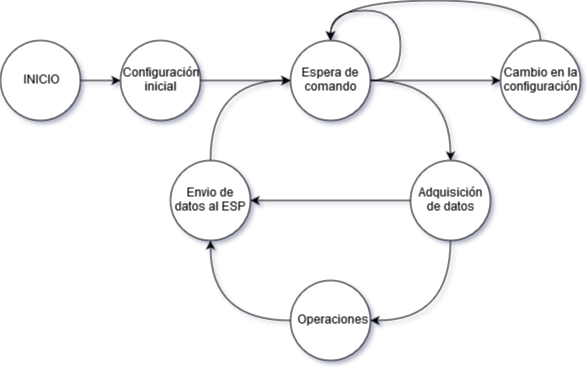
\includegraphics[width=16cm]{Maquina_estados_STM}
    \caption{Estructura del programa}
    \label{fig:Maquina_estados_STM}
\end{figure}

En primer lugar se realiza una inicialización de todas las variables, los periféricos y el resto de dispositivos que se encuentran conectados con el STM.

A continuación, el microcontrolador se queda a la espera de un comando por parte del ESP-12E que le indicará que hacer. Por el momento se han implementado tres alternativas, dos relacionadas con la adquisición de datos y una para cambios de   configuración, pero está preparado para aumentar el número de condiciones con facilidad. De esta forma el software puede aumentar en funcionalidades sin que haya que reestructurar el código.

Si el microcontrolador recibe la orden de adquirir datos, este activa la comunicación SPI y queda a la espera de una confirmación por parte del ADS de que los datos están listos para ser leídos del bus.

Tras leer los datos el microcontrolador convierte la información a formato \textit{float} y calcula la equivalencia en voltaje de la medida. 

Posteriormente, en función de la orden recibida desde el ESP, el STM transmite la información al ESP o bien realiza operaciones matemáticas sobre los datos y finalmente los transmite al ESP. Estas operaciones pueden ser sumas, restas e incluso un filtrado de la señal para eliminar componentes indeseadas.

\subsubsection{Transmisión de datos por SPI \label{sec:Software_micro_SPI}}

Aunque la capa de abstracción del hardware facilita notablemente el trabajo de desarrollo, para poder trabajar con un bus de comunicaciones de forma eficiente y sin errores es necesario saber como funciona a nivel hardware y, desde ahí, realizar una abstracción progresiva. 

En primer lugar será importante definir que elemento hará las funciones de Máster y cual de Esclavo, pues esto limitará las características de la comunicación y forzará la configuración de los \acrshort{GPIO} de una forma u otra.

\begin{figure} [h]
    \centering
    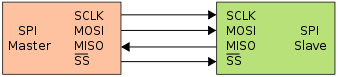
\includegraphics[width=10cm]{SPI_Master_Slave}
    \caption{Esquema de comunicaciones SPI}
    \label{fig:SPI_Master_Slave}
\end{figure}

Para aprovechar la tasa de transferencia del SPI del STM al máximo lo ideal sería que fuese este el Máster en ambas comunicaciones (hacia el ADS y hacia el ESP). Esto es así porque la máxima velocidad de transmisión es definida por el Máster mientras que el Esclavo se adapta a las normas impuestas, siempre dentro de unos rangos establecidos por el fabricante.

Por desgracia, las limitaciones de las librerías disponibles para el ESP-12E fuerzan que este sea obligatoriamente el Máster de esa comunicación limitando la velocidad a la máxima que sea capaz de alcanzar el ESP.

Para la transmisión de datos desde el STM es muy importante tener en cuenta que el microcontrolador trabaja a bajo nivel. Las funciones implementadas en los \textit{drivers} y librerías de abstracción de hardware facilitan el trabajo, pero debe tenerse presente en todo momento que se está transmitiendo información de registros de memoria y, por lo tanto, no se debe perder de vista el tamaño del dato ni el tipo del mismo.

Las funciones encargadas de transmitir información a través del puerto \acrshort{SPI} son:
\begin{itemize}
\item HAL\_StatusTypeDef HAL\_SPI\_Transmit
\item HAL\_StatusTypeDef HAL\_SPI\_Receive
\item HAL\_StatusTypeDef HAL\_SPI\_TransmitReceive
\end{itemize}

Las tres funciones necesitan el puntero al puerto por el que se transmitirá la información, la dirección de memoria de la misma, el tamaño del conjunto de datos y el tiempo de espera por cada transmisión.

El código \ref{algoritmo:STM_Transmision_SPI} muestra la cabecera de la función encargada de transmitir y recibir información de forma simultánea. En el se puede ver con claridad el tipo de datos que necesita para realizar una transmisión de datos de forma satisfactoria.

\begin{lstlisting}[label=algoritmo:STM_Transmision_SPI,style = STM-code,frame=single,caption=Transmisión de datos a través de SPI con el STM]
HAL_StatusTypeDef HAL_SPI_TransmitReceive(
	SPI_HandleTypeDef *hspi,
 	uint8_t *pTxData, 
 	uint8_t *pRxData, 
 	uint16_t Size, 
	uint32_t Timeout)
\end{lstlisting}

Las funciones encargadas de transmitir y recibir información, ya sea a través de SPI o a través de otro periférico, funcionan de forma similar y por lo tanto necesitan las mismas variables. Salta a la vista que, a pesar de que la función simplifica sensiblemente la gestión de memoria y pines, aún es necesario tener en cuenta ciertas limitaciones que marcarán el modo de trabajo:
\begin{itemize}
\item \textbf{Tamaño de transmisión fijo}\\
El tamaño de los datos a transmitir debe ser de 8 bits. En caso de querer transmitir una variable cuyo tamaño en memoria sea superior a este será necesario realizar una transformación.
\item \textbf{Gestión de pines manual o automática}\\
La gestión de pines como ``\textsc{Data-Ready}'' y ``\textsc{Start}'' se debe realizar de forma manual. ``\textsc{Chip-Select}'' en cambio está pensado para gestionarlo de forma manual o automática en función de las circunstancias.
\item \textbf{Gestión de memoria}\\
El STM es capaz de transmitir una gran cantidad de datos por \acrshort{SPI}. Es importante tener claro la cantidad de datos a recibir o transmitir, pues equivocarse puede suponer acceder a una dirección de memoria no permitida, recibir valores incorrectos o incluso corromper el código y forzar el reinicio del microcontrolador.
\end{itemize}

Al ser obligatorio transmitir datos de 8bits se vuelve indispensable crear algún metodo para poder dividir aquellas variables cuyos tamaño sea superior (float, long, etc).
El tipo de dato \textbf{union} definido en \textbf{C} está pensado justo para este cometido. Permite definir varias variables cuyo tamaño total sea equivalente y asignar la misma dirección de memoria a todas ellas. A continuación se muestra un fragmento del código necesario para dividir una variable \textbf{long} (32bits) en un array de 4 posiciones de tipo \textbf{int} (8bits cada una).

\begin{lstlisting}[label=algoritmo:STM_Divisor,style = STM-code,frame=single,caption=División de variables en otras de menor tamaño]
union miDato{
	struct
	{
		uint8_t  b[4];     // Array de bytes de tamaño equivalente
	}split;
		long dato;
} long_data; 
\end{lstlisting}
\clearpage

\subsubsection{Comunicación con el ADS \label{sec:Software_micro_ADS}}

El ADS está preparado para recibir y transmitir información a través del puerto SPI integrado. Aunque puede transmitir información el integrado sólo es capaz de actuar en modo Esclavo y \gls{Full Duplex}. Utilizando el microcontrolador STM como Master es posible comunicar ambos dispositivos a muy altas velocidades.

La memoria del ADS está organizada en distintos registros, cada uno de los cuales con una función definida en la hoja de características del componente. La configuración del dispositivo se realiza de forma casi exclusiva mediante SPI escribiendo directamente sobre el registro deseado.

Al tratarse de registros de memoria, para su modificación resulta indispensable conocer la posición exacta. Aunque para una máquina esto no es un problema, para un ser humano puede resultar complicado recordar e identificar de forma eficiente cada uno de ellos. 
\\Por este motivo se ha creado un archivo ``.h'' con definiciones de todos los registros, asociando cada uno de ellos a un comando. Así por ejemplo la posición de memoria encargada del control de los GPIO en lugar de llamarse escribiendo en el registro 0x14 basta con escribir en el registro \textsc{GPIO}. Con esta transformación se consigue además aumentar la legibilidad del código.

\begin{lstlisting}[label=algoritmo:STM_ADS_def,style = STM-code,frame=single,caption=Ejemplo de definiciones de los registros y funciones del ADS]
//Position in memory of registers: (Pg. 39)

#define ID 						0x00	// (0000 0000)
#define CONFIG1  		 	0x01	// (0000 0001) 
#define CONFIG2  			0x02 	// (0000 0010)
.		.						  .					.
#define CONFIG4   		0x17 	// (0001 0111)
\end{lstlisting}

El manual de funcionamiento del ADS muestra distintas formas de configuración. Es posible leer y/o escribir un registro o varios de forma simultánea con pocos comandos. De acuerdo al manual, para realizar una escritura de un registro es necesario transmitir tres datos al ADS. El primero indicará la dirección de memoria sobre la que se trabajará. El segundo sirve para seleccionar el número de registros a escribir. Por último el tercer dato es el que se almacenará en memoria. La figura \ref{fig:ADS_wreg} muestra una representación de la transmisión de datos llevada a cabo para la escritura de dos registros en el ADS:

\begin{figure} [h]
    \centering
    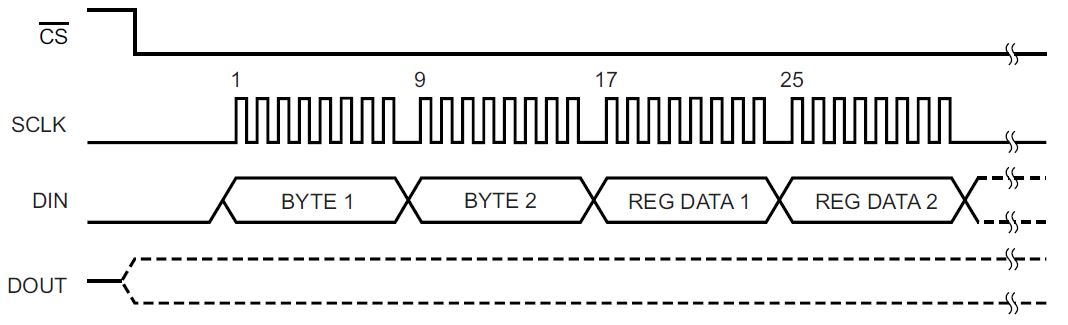
\includegraphics[width=13cm]{ADS_wreg}
    \caption{Escritura de dos registros del ADS \cite{Datasheet_ADS}}
    \label{fig:ADS_wreg}
\end{figure}

El código generado en el STM para realizar esta función es el presentado en \ref{algoritmo:STM_wreg}.

\begin{lstlisting}[label=algoritmo:STM_wreg,style = STM-code,frame=single,caption=Escritura en registros del ADS]
void adc_wreg(uint8_t reg, uint8_t val, SPI_HandleTypeDef *SPI){
	uint8_t zero_t = 0x00;
	uint8_t zero_r = 0x00;
	uint8_t reg_temp = WREG | reg;
	uint8_t val_temp = val;
	
	HAL_GPIO_WritePin(A_CS0_N_GPIO_Port, A_CS0_N_Pin, GPIO_PIN_RESET);
	HAL_SPI_TransmitReceive(SPI, &reg_temp, &zero_r, 1, 100);
	HAL_SPI_TransmitReceive(SPI, &zero_t, &zero_r, 1, 100);	
	HAL_SPI_TransmitReceive(SPI, &val_temp, &zero_r, 1, 100);	

	HAL_Delay(1);
	HAL_GPIO_WritePin(A_CS0_N_GPIO_Port, A_CS0_N_Pin, GPIO_PIN_SET);
}
\end{lstlisting}

La lectura de los registros del ADS se realiza de una forma análoga. En esta ocasión se transmiten los mismos dos datos que para escribir en un registro siendo la única diferencia que el tercer dato (y los siguientes en caso de ser más de un registro) se transmitirán desde el ADS hacia el STM tal y como aparece en la figura \ref{fig:ADS_rreg}.

\begin{figure} [h]
    \centering
    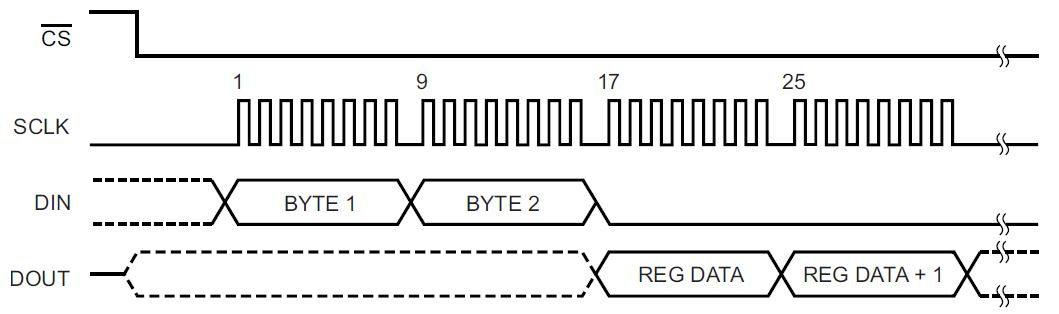
\includegraphics[width=13cm]{ADS_rreg}
    \caption{Lectura de dos registros del ADS \cite{Datasheet_ADS}}
    \label{fig:ADS_rreg}
\end{figure}

\begin{lstlisting}[label=algoritmo:STM_rreg,style = STM-code,frame=single,caption=Lectura de registros del ADS]
uint8_t adc_rreg(uint8_t reg, SPI_HandleTypeDef *SPI){
	uint8_t val = 0x00;
	uint8_t zero_t = 0x00;
	uint8_t zero_r = 0x00;
	uint8_t temp = RREG | reg;
	
	HAL_GPIO_WritePin(A_CS0_N_GPIO_Port, A_CS0_N_Pin, GPIO_PIN_RESET);
	HAL_SPI_TransmitReceive(SPI, &temp, &zero_r, 1, 100);
	HAL_SPI_TransmitReceive(SPI, &zero_t, &zero_r, 1, 100);	
	HAL_SPI_TransmitReceive(SPI, &zero_t, &val, 1, 100);

	HAL_Delay(1);
	HAL_GPIO_WritePin(A_CS0_N_GPIO_Port, A_CS0_N_Pin, GPIO_PIN_SET);

	return val;
}
\end{lstlisting}

Para que la transmisión sea correcta es muy importante que todas las variables definidas sean independientes. Además, el ADS necesita que durante la lectura de datos el pin \textsc{MOSI} se mantenga en un 0 lógico todo el rato.

\subsubsection{Lectura y conversión de datos \label{sec:Software_micro_Datos}}

El ADS está construído utilizando un sistema adquisidor de 8 canales, todos adquiridos de forma simultánea utilizando un sistema $\Delta\Sigma$ de 24 bits y ganancia variable.

Tras adquirir los datos estos son codificados siguiendo el siguiente formato:
\begin{table} [H]
 \centering
 \begin{tabular}{|c|c|}
 \hline 
\textbf{Señal de entrada, V$_{IN}$} &  \multirow{2}{*}{\textbf{Código de salida ideal}}\\ 
 \textbf{(INxP - INxN)} &  \\ 
 \hline 
 +FS & 7FFFFFh\\ 
 \hline 
 +FS$/(2^{23}-1)$ & 000001h \\ 
 \hline 
 0 & 000000h\\ 
 \hline 
 -FS & FFFFFFh\\ 
 \hline 
 +FS$(2^{23}/(2^{23}-1))$ & 800000 \\ 
 \hline 
 \end{tabular} 
 \caption{Equivalencia de voltaje ideal de entrada y código de salida}
 \label{tab:ADS_equivalencia}
\end{table}

La tabla anterior es una modificación de la proporcionada en la hoja de características del ADS corrigiendo algunas pequeñas erratas. La variable ``FS'' corresponde a la escala completa de entrada del ADS. En este caso son 4.5V divididos por la ganancia (G).

Para \textbf{voltajes positivos} la decodificación de estos valores es muy sencilla, pues basta con aplicar una simple \textbf{regla de tres} en la que cada bit es un incremento de $4.5V/(2^{23}*G)$.\\
Para \textbf{voltajes negativos} basta con \textbf{invertir} todos los bits y aplicar la misma regla de tres.\\
El bit más significativo indica si el voltaje final será positivo (0) o negativo (1) y es el que se ha usado como referencia para aplicar la conversión anterior en caso de ser necesaria.

Al trabajar con datos de 24 bits no es posible realizar una inversión directa del valor de la variable o los 8 bits más significativos se verían invertidos también. Por suerte el ADS transmite los datos en paquetes de 8 bits lo cual facilita tratarlos de forma independiente y, tras hacer la transformación a nivel de bit, crear una variable que represente el valor real.

Unir los tres bytes una vez se ha realizado la conversión es posible de múltiples formas. Por motivos de eficiencia y de reutilización del código se ha realizado la misma aproximación ya expuesta previamente haciendo uso de datos de tipo \textbf{union}.

El código \ref{algoritmo:ADS_decodificacion}, incluído en una librería creada para interactuar con el ADS, es el utilizado para este fin.

\clearpage

\begin{lstlisting}[label=algoritmo:ADS_decodificacion,style = STM-code,frame=single,caption=Decodificación de datos binarios a Voltajes]
float32_t byte2float (uint8_t data_23_16, uint8_t data_15_8, uint8_t data_7_0, uint8_t ganancia)
	{
		float32_t value = 0;
		
		union miDato{
		struct
		{
			uint8_t  b[4];     // Array de bytes de tamaño igual al tamaño de la primera variable: int = 2 bytes, float = 4 bytes
		}split;
			long dato;
	 } long_data; 
		
	 long_data.dato = 0;
	 
		if (data_23_16>=0x80) //1000 0000
		{
			long_data.split.b[2] = ~data_23_16;
			long_data.split.b[1] = ~data_15_8;
			long_data.split.b[0] = ~data_7_0;
			value = long_data.dato;
			value = -value;
		}
		else
		{
			long_data.split.b[2] = data_23_16;
			long_data.split.b[1] = data_15_8;
			long_data.split.b[0] = data_7_0;
			value = long_data.dato;
		}
		
		value = value*4.5f/(8388607.0f*ganancia); //4.5/(2^23*G)
		
		return value;
	}
\end{lstlisting}

El código anterior realiza una conversión triple: 4 bytes $\Rightarrow$ long $\Rightarrow$ float, donde el valor final devuelto es el voltaje real medido una vez se ha aplicado el factor de ganancia correspondiente.

El ADS tiene embebido un sistema de control basado en comandos a través de SPI. Estos comandos permiten realizar ciertas operaciones en tiempo real que facilitan el control del integrado y amplian sus características. 

La tabla \ref{tab:ADS_comandos}, sacada de la hoja de características del componente, muestra todos los comandos que el ADS es capaz de reconocer, sus funciones y el conjunto de bytes que representa cada uno. Los últimos dos comandos corresponden a la lectura y escritura en registros y ya han sido explicados previamente.

\begin{table}[H]
    \centering
    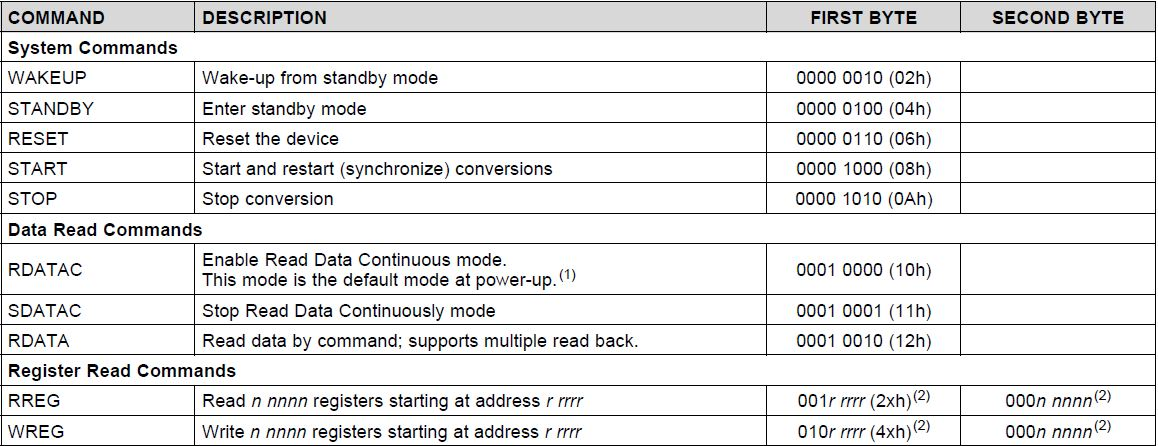
\includegraphics[width=16cm]{ADS_comandos}
    \caption{Comandos del ADS1299}
    \label{tab:ADS_comandos}
\end{table}

Durante la realización de este proyecto ha sido necesario utilizar la mayor parte de los comandos presentados en la tabla anterior. Cabe destacar que aquellos categorizados como ``Comandos del sistema'' han sido necesarios durante la secuencia de inicio del ADS casi en exclusiva, pues no se han implementado funciones de ahorro de energía. Estas se han contemplado como una mejora a llevar a cabo en futuras iteraciones de este proyecto.

El ADS cuenta con dos modos de lectura: continua y bajo demanda. Los comandos categorizados como ``Comandos de lectura'' están relacionados con la gestión de estos dos modos y se dividen a su vez en dos tipos según su función:
\begin{itemize}
\item \textbf{Configuración}\\
\textsc{RDATAC} y \textsc{SDATAC} activan y desactivan el modo de lectura continua respectivamente. El ADS se encuentra por defecto en modo continuo tras completar la secuencia de inicio.
\item \textbf{Lectura}\\
\textsc{RDATA} solicita en el modo de lectura bajo demanda la transmisión de los datos capturados en ese momento.
\end{itemize} 

El modo bajo demanda está pensado para aquellos sistemas en los que es necesario adquirir poca información a lo largo del tiempo. En esta configuración el ADS se mantiene inactivo hasta que recibe el comando de lectura y sólo entonces es cuando la realiza. Este comportamiento favorece la implementación de sistemas de ahorro de energía basados en los comandos \textsc{STANDBY} y \textsc{WAKEUP}. De esta forma es posible aumentar la autonomía del sistema completo considerablemente.

Por desgracia, este modo no es compatible con la transmisión de grandes cantidades de datos o mediciones muy continuas. Por cada medida es necesario utilizar el comando \textsc{RDATA}, afectando directamente al rendimiento y eficiencia en la transmisión.

La figura \ref{fig:ADS_SDATAC} ilustra la transmisión de información usando el modo bajo demanda.

\begin{figure} [H]
    \centering
    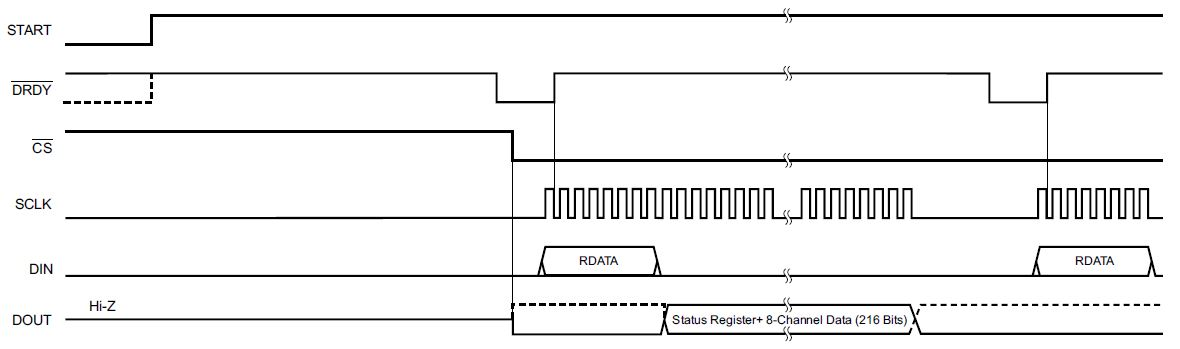
\includegraphics[width=15cm]{ADS_SDATAC}
    \caption{Modo de uso del comando \textsc{RDATA}}
    \label{fig:ADS_SDATAC}
\end{figure}

Por los motivos explicados anteriormente este modo no será utilizado normalmente pero aún así se ha decidido trabajar en su implementación en caso de que fuese necesario en el futuro. El código utilizado para adquirir datos es el siguiente:

\begin{lstlisting}[label=algoritmo:ADS_oneshot,style = STM-code,frame=single,caption=Lectura de datos en modo \textit{one-shot}]
void one_shot (uint8_t data[], SPI_HandleTypeDef *SPI)
{
	uint8_t zero = 0x00;
	uint8_t cmd = RDATA;
			
	while (HAL_GPIO_ReadPin(A_DRDY_N_GPIO_Port, A_DRDY_N_Pin) == GPIO_PIN_SET){}

	HAL_GPIO_WritePin(A_CS0_N_GPIO_Port, A_CS0_N_Pin, GPIO_PIN_RESET);
	
	HAL_SPI_TransmitReceive(SPI, &cmd, &zero,  1, 100);

	read_data_frame(data, SPI);
			
	while (HAL_GPIO_ReadPin(A_DRDY_N_GPIO_Port, A_DRDY_N_Pin) == GPIO_PIN_RESET) {}			
				
	HAL_GPIO_WritePin(A_CS0_N_GPIO_Port, A_CS0_N_Pin, GPIO_PIN_SET);

	update_bias_ref(data, SPI);
}
\end{lstlisting}

Para recibir una gran cantidad de información de forma ininterrumpida el ADS cuenta con el modo continuo. Se transmite el comando \textsc{RDATAC} y desde ese momento el ADS empieza a adquirir información y transmitirla. El pin \textsc{DRDY} es utilizado por el ADS para indicar que la siguiente tanda de datos está disponible para su lectura. 

La figura \ref{fig:ADS_RDATAC} representa la transmisión de información en modo continuo y el código \ref{algoritmo:ADS_continuo} el código equivalente.

\begin{figure} [H]
    \centering
    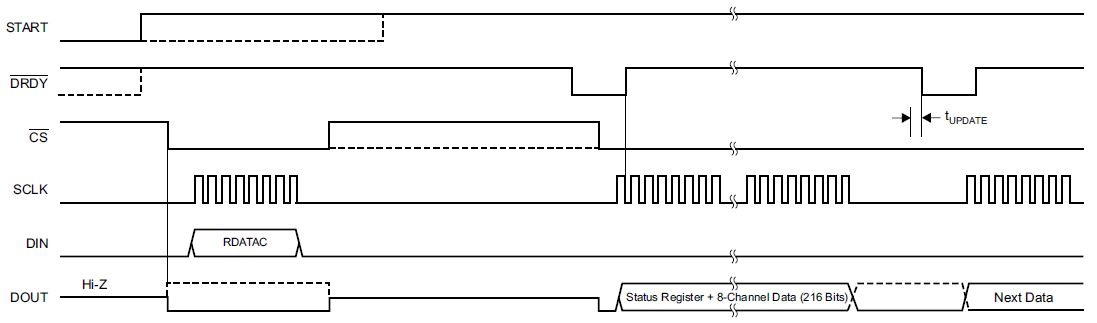
\includegraphics[width=16cm]{ADS_RDATAC}
    \caption{Transmisión de datos en modo continuo}
    \label{fig:ADS_RDATAC}
\end{figure}

\begin{lstlisting}[label=algoritmo:ADS_continuo,style = STM-code,frame=single,caption=Lectura de datos en modo continuo]
void adquire_array_data (uint8_t data[], float32_t channel_1[],float32_t channel_2[],float32_t channel_3[],float32_t channel_4[],float32_t channel_5[],float32_t channel_6[],float32_t channel_7[],float32_t channel_8[], uint8_t gain[], SPI_HandleTypeDef *SPI)
{
	int debug = 255;
	// read LENGTH_SAMPLES samples
		
	adc_send_command(RDATAC, SPI);
		
	while (HAL_GPIO_ReadPin(A_DRDY_N_GPIO_Port, A_DRDY_N_Pin) == GPIO_PIN_SET){}
		
	HAL_GPIO_WritePin(A_CS0_N_GPIO_Port, A_CS0_N_Pin, GPIO_PIN_RESET);
		
	read_data_frame(data, SPI);
			
	channel_1[0]=byte2float(data[1*3], data[1*3+1], data[1*3+2], gain[0]);
	channel_2[0]=byte2float(data[2*3], data[2*3+1], data[2*3+2], gain[1]);
	channel_3[0]=byte2float(data[3*3], data[3*3+1], data[3*3+2], gain[2]);
	channel_4[0]=byte2float(data[4*3], data[4*3+1], data[4*3+2], gain[3]);
	channel_5[0]=byte2float(data[5*3], data[5*3+1], data[5*3+2], gain[4]);
	channel_6[0]=byte2float(data[6*3], data[6*3+1], data[6*3+2], gain[5]);
	channel_7[0]=byte2float(data[7*3], data[7*3+1], data[7*3+2], gain[6]);
	channel_8[0]=byte2float(data[8*3], data[8*3+1], data[8*3+2], gain[7]);
			
	while (HAL_GPIO_ReadPin(A_DRDY_N_GPIO_Port, A_DRDY_N_Pin) == GPIO_PIN_RESET){}
			
	for (int i = 1; i<LENGTH_SAMPLES; i++)
	{
		while (HAL_GPIO_ReadPin(A_DRDY_N_GPIO_Port, A_DRDY_N_Pin) == GPIO_PIN_SET){}
			
		read_data_frame(data, SPI);

		channel_1[i]=byte2float(data[1*3], data[1*3+1], data[1*3+2], gain[0]);
		channel_2[i]=byte2float(data[2*3], data[2*3+1], data[2*3+2], gain[1]);
		channel_3[i]=byte2float(data[3*3], data[3*3+1], data[3*3+2], gain[2]);
		channel_4[i]=byte2float(data[4*3], data[4*3+1], data[4*3+2], gain[3]);
		channel_5[i]=byte2float(data[5*3], data[5*3+1], data[5*3+2], gain[4]);
		channel_6[i]=byte2float(data[6*3], data[6*3+1], data[6*3+2], gain[5]);
		channel_7[i]=byte2float(data[7*3], data[7*3+1], data[7*3+2], gain[6]);
		channel_8[i]=byte2float(data[8*3], data[8*3+1], data[8*3+2], gain[7]);
				
		while (HAL_GPIO_ReadPin(A_DRDY_N_GPIO_Port, A_DRDY_N_Pin) == GPIO_PIN_RESET){}
	}
		
	HAL_GPIO_WritePin(A_CS0_N_GPIO_Port, A_CS0_N_Pin, GPIO_PIN_SET);
}
\end{lstlisting}

El STM no permite trabajar con vectores de varias dimensiones de la misma forma que otros lenguajes de programación, así que para capturar todos los canales ha sido necesario repetir código. A cambio, el escalado del código de un canal a varios se realiza de una forma sencilla e intuitiva. En posteriores revisiones de este proyecto se valorará su sustitución por otro sistema más eficiente.

\subsubsection{DSP - Implementación de filtros \label{sec:Software_micro_DSP}}

Una de las características que diferencian los microcontroladores de esta familia de los de otras es la capacidad de realizar operaciones matemáticas sin que ello repercuta de forma muy significativa en el rendimiento. 

Para facilitar su utilización y unificar a todos los desarrolladores ARM ha creado una librería llamada CMSIS-DSP que engloba todas las funcionalidades de procesado de señal más comunes, optimizando dichos algoritmos para hacerlos lo más eficientes posible.
Esta librería incluye los siguientes tipos de operaciones:

\begin{itemize}
\item Operaciones matemáticas básicas, rápidas y complejas
\item \textbf{Filtrado}
\item Matrices
\item Transformaciones
\item Estadísticas
\item Controladores (PID, senos, etc)
\item Interpolación
\item Apoyo
\end{itemize}

Estas funciones utilizan variables de tipo enteros de 8, 16 y 32 bits y float de 32 bits. En esta ocasión se han utilizado exclusivamente las funciones de filtrado de señal, concretamente aquellas dedicadas a la realización de filtros FIR y su aplicación a señales.

ARM ha puesto a disposición de los consumidores una página web de referencia en la que se puede encontrar una descripción detallada de cada función incluyendo su modo de uso y ejemplos \cite{CMSIS-DSP}.

El filtrado de una señal con un filtro FIR en ARM es un proceso sencillo pero que engloba varias herramientas, pues el diseño del filtro se debe realizar de forma independiente. La función utilizada para este fin es ``arm\_fir\_f32()''. \\
Esta función recibe una señal en formato \textbf{float32\_t} (x[n]), los coeficientes del filtro y la longitud de la ventana y devuelve una señal filtrada (y[n]) con las características deseadas.
\begin{figure} [h]
    \centering
    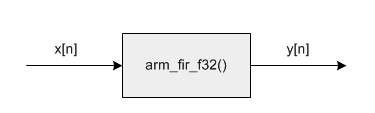
\includegraphics[width=7cm]{arm_fir_f32}
    \caption{Diagrama de bloques del filtrado de una señal x[n]}
    \label{fig:arm_fir_f32}
\end{figure}

El código necesario para aplicar un filtro FIR a una señal es el siguiente:

\begin{lstlisting}[label=algoritmo:STM_filtro,style = STM-code,frame=single,caption=Filtro FIR en STM]
/* ----------------------------------------------------------------------
** Includes necesarios
** ------------------------------------------------------------------- */
#include "arm_math.h"
#include "math_helper.h"
const float32_t firCoeffs32[NUM_TAPS] = {h1, h2, ....,hn}
/* ------------------------------------------------------------------
 * Variables globales para el filtro FIR
 * ------------------------------------------------------------------- */
uint32_t blockSize = BLOCK_SIZE;
uint32_t numBlocks = TEST_LENGTH_SAMPLES/BLOCK_SIZE;
 * ------------------------------------------------------------------- */
arm_fir_instance_f32 S;
arm_status status;
float32_t  *inputF32, *outputF32;
/* Inicialización de buffers de entrada y salida */
inputF32 = &testInput_f32_1kHz_15kHz[0];
outputF32 = &testOutput[0];
/* Inicialización de la estructura de la instancia del filtro FIR. */
arm_fir_init_f32(&S, NUM_TAPS, (float32_t *)&firCoeffs32[0], &firStateF32[0], blockSize);
/* ----------------------------------------------------------------------
** Aplicación del filtro a cada conjunto de blockSize
** ------------------------------------------------------------------- */
for(i=0; i < numBlocks; i++)
{
  arm_fir_f32(&S, inputF32 + (i * blockSize), outputF32 + (i * blockSize), blockSize);
}
\end{lstlisting}

Es una función muy versátil que permite, entre otras cosas, preparar un gran número de filtros y utilizar el más adecuado para cada ocasión sin apenas cambiar el código.

Una de las componentes en frecuencia que más afecta a todas las señales es la de 50 Hz. Para su eliminación se hace uso del equivalente a un filtro \textit{Notch} implementado en un filtro \acrshort{FIR}. Esto se consigue creando un filtro de rechazo de banda lo suficientemente estrecho como para que afecte poco a frecuencias cercanas a la frecuencia a eliminar.

El diseño del filtro se puede hacer con cualquiera de las herramientas disponibles en MatLab. La función ``fir1'' es capaz de definir un filtro con cualquier característica. Tras una primera aproximación con esa función se consiguió un filtro con la respuesta en frecuencia de la figura \ref{fig:FIR_fir1}.
\begin{figure} [H]
    \centering
    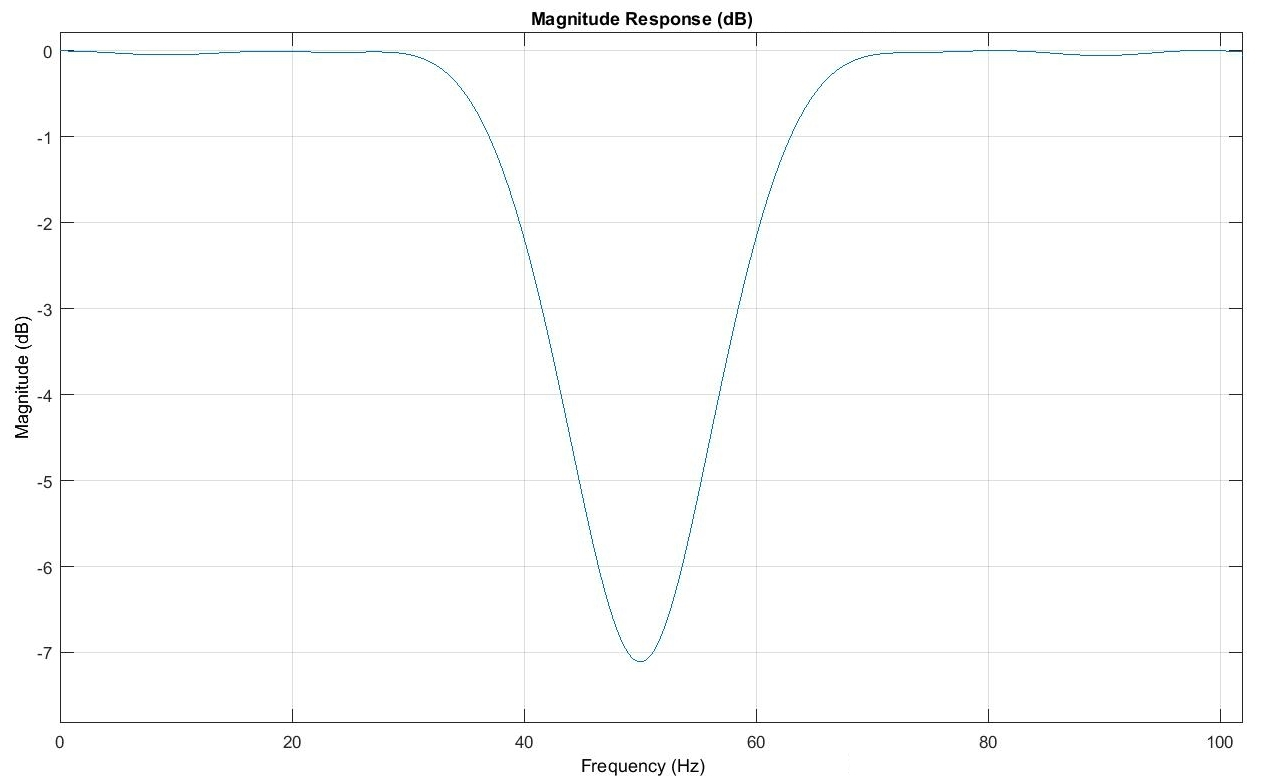
\includegraphics[width=15cm]{FIR_fir1}
    \caption{Respuesta en frecuencia del filtro definido con fir1}
    \label{fig:FIR_fir1}
\end{figure}

Este filtro presenta un comportamiento similar al esperado y un rizado apenas apreciable pero con un factor de rechazo muy bajo. Utilizando otra herramienta diseñada por F.S. Schlindwein disponible en el \textit{workshop} de MatLab es posible ajustar aún más el filtro sin apenas esfuerzo. Tras un par de iteraciones el resultado final fue

\begin{figure} [H]
    \centering
    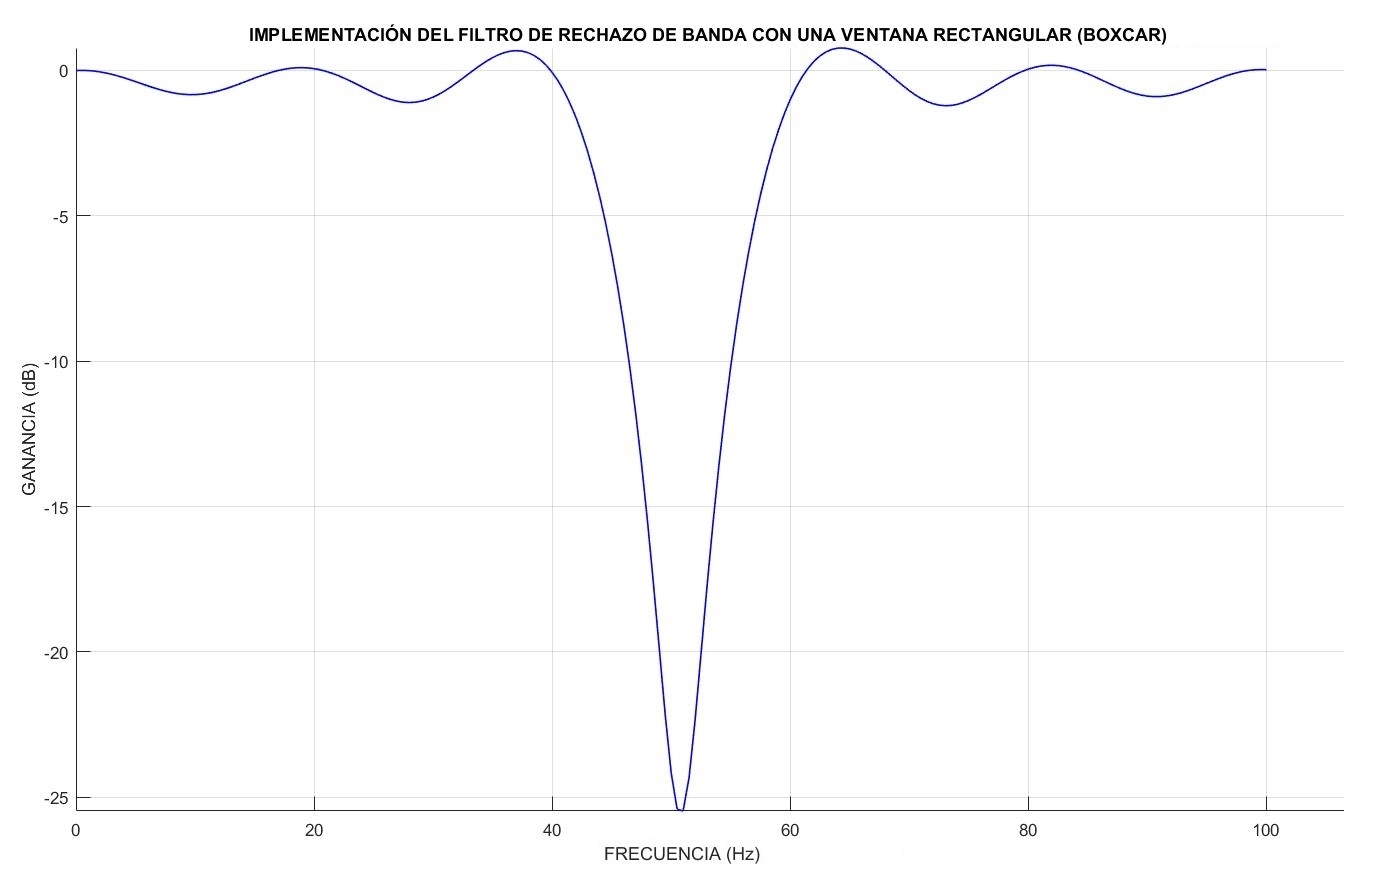
\includegraphics[width=13cm]{NOTCH_50Hz}
    \caption{CAPTION}
    \label{fig:NOTCH_50Hz}
\end{figure}


Por desgracia la utilización de esta librería provoca que el código supere las limitaciones de la versión gratuita de Keil haciendo necesaria una licencia para poder compilar.

\subsubsection{Comunicación con el ESP \label{sec:Software_micro_ESP}}

El código \ref{algoritmo:STM_Transmision_SPI} es el utilizado para transmitir información al ESP y recibirla.

\begin{lstlisting}[label=algoritmo:STM_Transmision_SPI,style = STM-code,frame=single,caption=Transmisión de datos a través de SPI con el STM]
uint8_t commandFromESP(uint8_t command, SPI_HandleTypeDef *hspi1)
{
	uint8_t response = 0x00;	

		HAL_GPIO_WritePin(DRDY_N_GPIO_Port,DRDY_N_Pin, GPIO_PIN_RESET);
		HAL_SPI_TransmitReceive(hspi1, &command, &response, 1, 100);
		HAL_GPIO_WritePin(DRDY_N_GPIO_Port,DRDY_N_Pin, GPIO_PIN_SET);
		HAL_GPIO_TogglePin(LED_GPIO_Port,LED_Pin); 	//LED OFF
		HAL_Delay(50);
	
	return response;
}
\end{lstlisting}

\subsubsection{Programación del microcontrolador\label{sec:Software_micro_ESP}}

%Software
%Microcontrolador STM
%	CubeMX
%	HAL
%	Implementación del Firmware
%		Maquina de estados
%		Transmisión de datos por SPI
%		Comunicación con ADS
%		Lectura y conversión de datos
%		DSP - Implementación de filtros
%		Comunicación con el ESP
%		
%Microcontrolador ESP
%	Arduino
%	Configuración 
%	Firmware
%		Maquina de estados
%		Transmisión de datos por SPI
%		Comunicación con el STM
%
%LabView
